\documentclass[letterpaper,10pt]{article}

%\setlength{\parindent}{0in}
%\usepackage{fullpage} 
\usepackage{amsmath}
\usepackage{amssymb}
\usepackage{enumerate}
\usepackage{graphicx}
\usepackage[table]{xcolor}
\usepackage{dcolumn}
\oddsidemargin 0.0in
\textwidth 6.5in
\newcolumntype{.}{D{.}{.}{-1}}
\newcommand*{\myalign}[2]{\multicolumn{1}{#1}{#2}}

%opening
\title{Homework}
\author{Steve Mazza}
\date{July 22, 2013}

\begin{document}
\maketitle

\section*{Homework 4}
\subsection*{Problem 1}
\subsubsection*{(a)}
\begin{align*}
	G(s) &= \dfrac{50}{(s+1)(s+5)(s+50)} \\
	G(s) &= \dfrac{0.2}{\left(1+\dfrac{s}{1}\right)\left(1 + \dfrac{s}{5}\right)\left(1 + \dfrac{s}{50}\right)} \\
	\mbox{decay constants} &= 1;5;10 \\
	G_{simpl}(s) &= \dfrac{0.2}{s+1}
\end{align*}
\subsubsection*{(b)}
\begin{align*}
	G(s) &= \dfrac{100}{(s+1)(s^2+12s+20)} \\
	G(s) &= \dfrac{5}{\left(1+\dfrac{s}{1}\right)\left(1+\dfrac{3}{5}s+\dfrac{s^2}{20}\right)} \\
	\mbox{decay constants} &= 0.6;1\\
	G_{simpl}(s) &= \dfrac{100}{\left(s^2+12s+20\right)}
\end{align*}
\subsubsection*{(c)}
\begin{align*}
	G(s) &= \dfrac{10}{(s+5)(s^2+2s+2)(s^2+4)} \\
	G(s) &= \dfrac{0.25}{\left(1+\dfrac{s}{5}\right)\left(1+s+\dfrac{s^2}{4}\right)\left(1+\dfrac{S^2}{4}\right)} \\
	\mbox{decay constants} &= 0;1;5 \\
	G_{simpl}(s) &= \dfrac{2}{\left(s^2+2s+2\right)\left(s^2+4\right)}
\end{align*}
\subsubsection*{(d)}
\begin{align*}
	G(s) &= \dfrac{72(s+8)}{(s+4)(s+12)(s^2+8s+12)} \\
	G(s) &= \dfrac{1\times\left(1+\dfrac{s}{8}\right)}{\left(1+\dfrac{s}{4}\right)\left(1+\dfrac{s}{12}\right)\left(1+\dfrac{2s}{3}+\dfrac{s^2}{12}\right)} \\
	\mbox{decay constants} &= 0.\overline{66};4;12 \\
	G_{simpl}(s) &= \dfrac{12}{s^2+8s+12}
\end{align*}

\subsection*{Problem 2}
\subsubsection*{(a)}
\begin{center}
	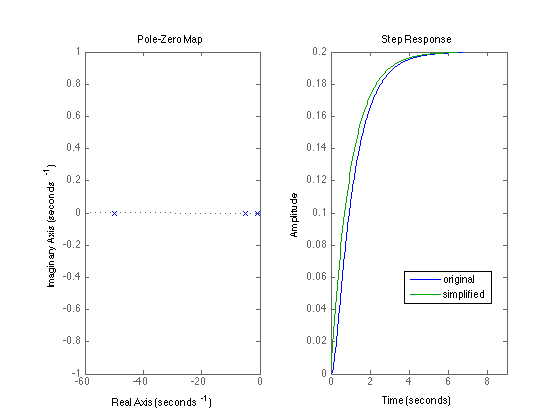
\includegraphics[scale=0.5]{homework03-2a.png}
\end{center}
\subsubsection*{(b)}
\begin{center}
	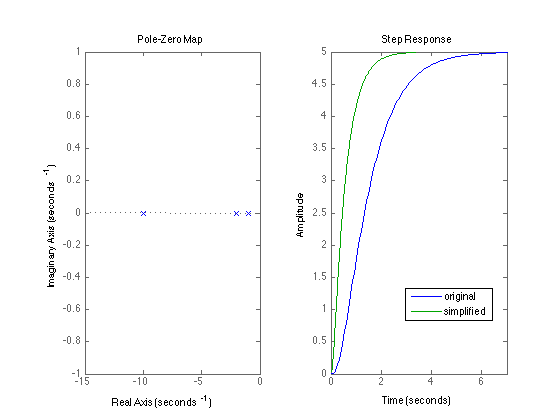
\includegraphics[scale=0.5]{homework03-2b.png}
\end{center}
\subsubsection*{(c)}
\begin{center}
	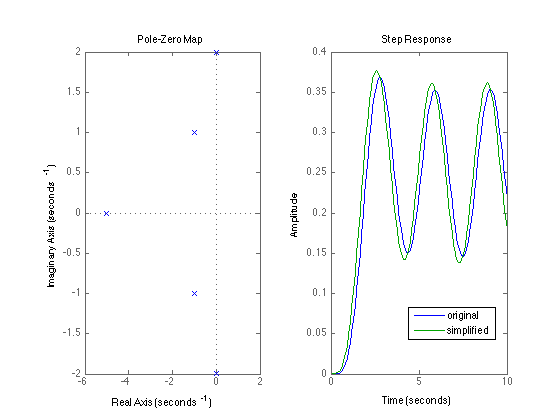
\includegraphics[scale=0.5]{homework03-2c.png}
\end{center}
\subsubsection*{(d)}
\begin{center}
	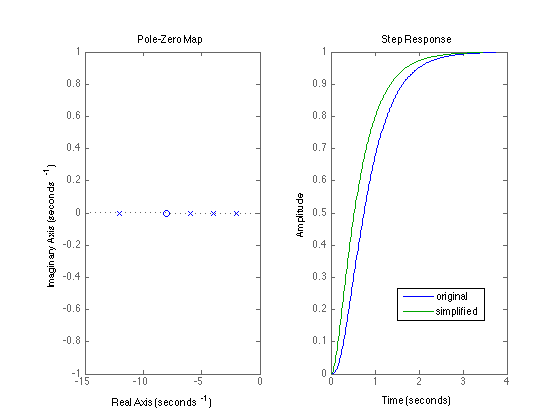
\includegraphics[scale=0.5]{homework03-2d.png}
\end{center}
Please see the attached file for MATLAB code.

\subsection*{Problem 4}
Applying the negative feedback rule, $C(s) = \dfrac{G(s)}{1-G(s)H(s)}R(s)$ twice, we obtain a transfer function for the simplified block diagram, \[ \dfrac{100}{s^2 + 100Ks + 100}\]  We then proceed to solve for $\omega_{n}$,
\begin{align*}
	\omega_{n} &= \sqrt{100} \\
	\omega_{n} &= 10 
\end{align*}
and $\zeta$,
\begin{align*}
	100K &= 2\zeta\omega_{n} \\
	50K &= 10\zeta \\
	\zeta &= 5K
\end{align*}
To achieve a zero overshoot and as rapid a response time as possible, we select $\zeta = 1$, or \emph{critical damping}, from which we derive $K$,
\begin{align*}
	\zeta &= 5K \\
	1 &= 5K \\
	K &= 0.2 
\end{align*}
Assuming a Type 2 system, we determine our steady-state error from the formula  $E_{ss} = \dfrac{1}{K} = 5$.

\section*{Homework 5}
\subsection*{Problem 1}
\subsubsection*{(a)}
\begin{tabular}{cc}
	1&6\\
	4&6\\
	9/2&\\
	6&
\end{tabular}\\
$s^3+4s^2+6s+6$ is stable.  There are no roots in the right-hand plane.
\subsubsection*{(b)}
\begin{tabular}{cc}
	1&$2+K$\\
	$3K$&5\\
	$K+2-5/3K$&\\
	5&
\end{tabular}\\
$s^3+3Ks^2+(2+K)s+5$ is stable for approximate values of $K, -2.63 < K < 0$ and $K > 0.63$.  The number of roots in the right-hand plane will be determined by the value of $K$.
\subsubsection*{(c)}
\begin{tabular}{ccc}
	1&2&8\\
	1&10&\\
	-8&8&\\
	11&&\\
	8&&
\end{tabular}\\
$s^4+s^3+2s^2+10s+8$ is unstable.  There are 2 roots in the right-hand plane.
\subsubsection*{(d)}
\begin{tabular}{ccc}
	1&3&$K$\\
	1&2&\\
	1&$K$&\\
	$2-K$&&\\
	$K$&&
\end{tabular}\\
$S^4+s^3+3s^2+2s+K$ is stable for $K, 0<K<2$.  The number of roots in the right-hand plane will be determined by the value of $K$.
\subsubsection*{(e)}
\begin{tabular}{ccc}
	1&2&11\\
	1&0&5\\
	2&-4&\\
	2&5&\\
	-9&&\\
	5&&
\end{tabular}\\
$s^5+s^4+2s^3+s+5$ is unstable.  There are 2 roots in the right-hand plane.
\subsubsection*{(f)}
\begin{tabular}{ccc}
	1&2&1\\
	1&1&$K$\\
	1&$1-K$&\\
	$K$&$K$&\\
	$-K$&&\\
	$K$&&
\end{tabular}\\
$s^5+s^4+2s^3+s^2+s+K$ is unstable.  There are 2 roots in the right-hand plane.

\subsection*{Problem 4}
We simplify the block diagram to obtain
\[G(s) = \dfrac{\omega_{n}^{2}}{s(s+2\zeta\omega_{n})+\omega_{n}^{2}}\]
Then we continue as follows,
\begin{align*}
	\dfrac{C(s)}{R(s)} &= \dfrac{\omega_{n}^{2}(1+T_{d}s)}{s(s+2\zeta\omega_{n})+\omega_{n}^{2}} \\
	\dfrac{E(s)}{R(s)} &= 1 - \dfrac{\omega_{n}^{2}(1+T_{d}s)}{s(s+2\zeta\omega_{n})+\omega_{n}^{2}} \\
	E(s) &= \dfrac{1}{s^2} \left[ \dfrac{s^2+2\zeta\omega_{n}s-T_{d}s\omega_{n}^{2}}{s^2+2\zeta\omega_{n}s+\omega_{n}^{2}} \right] \\
	\lim_{s\to0}sE(s) &= \dfrac{2\zeta\omega_{n}-T_{d}\omega_{n}^{2}}{\omega_{n}^{2}} \\
	&= \dfrac{2\zeta-T_{d}s\omega_{n}}{\omega_{n}}
\end{align*}
And so it turns out that the \emph{proper} value for $T_{d}$ is, in fact, $\dfrac{2\zeta}{\omega_{n}}$.

\end{document}